\section{Introducción}

Desde inicios del milenio, la población en América Latina ha tenido un crecimiento semejante a una exponencial\cite{CEPAL_2015}. Esto genera problemas de aglomeración urbana, distribución de suelo, movilidad urbana privdo y público, entre otros. Las metrópolis de América Latina tienen retos difíciles, ya que sus problemas se ven reflejados en el tiempo y distancia de traslado que realiza cada habitante\cite{hall_1978}. Por lo que el problema de transporte y movilidad urbana es uno de los factores más importantes para las administraciones, siendo un pilar fundamental en el desarrollo social y económico. La aplicación del principio de comodalidad plantea favorecer la promoción e implementación de distintas alternativas que satisfagan las necesidades de transporte, garantizando cobertura, conectividad, flujos continuos, seguridad y eficiencia\cite{pastori_2018}.

Frente a estos problemas en el transporte público, varias metrópolis de América Latina han comenzado a implementar el principio de comodalidad. La bicicleta es un medio de transporte alternativo, que dependiendo la implementación, puede llegar a ser más rápido, comodo y seguro en comparación a los demás medios de transporte disponibles.

La congestión del tráfico en las grandes ciudades presentan graves problemas de movilidad. Entre las causas que crean esta congestión son la falta de planeación y la desarrollo en la infraestructura y la alta densidad poblacional. Una correcta implementación de un sistema de bicicletas aporta a la disminución de la congestión del tráfico.

En el mundo existen alrededor de 400 sistemas de bicicletas disponibles al público. Cada sistema tiene particulariades y tecnologias que se ajustam a las necesidades de la región y habitantes. La implementación de estos sistemas se debe realizar sobre un estudio que incluye diferentes factores para que se aporte de una manera eficiente hacia la disminución del tráfico.

\section{Antecedentes}

El área metropolitana de la Ciudad de México tiene un sistema de transporte público que intregra 11 línea de metro, 7 de autobuses (Metrobus), autobuses no integrados y sistema de bicicleta público.

\textit{ECOBICI} es el sistema de bicicletas públicas compartidas de la Ciudad de México. El sistema permite que a los usuarios registrados tomar una bicicleta de cualquier estación y devolverla a la más cercana a su destino en trayectos de 45 minutos.

\section{MIBICI}

Guadalajara es la segunda metrópolis más importante de México. Su sistema de transporte incluye 2 lineas de tren ligero, una linea de autobuses integrados, autobuses no integrados y el sistema de bicis público \textit{MIBICI}.

MIBICI es el sistema público de bicicletas de la ciudad de Guadalajara. Es un sistema el cual esta diseñado para realizar recorridos cortos de manera eficiente tomando en cuenta los siguientes puntos:

\begin{itemize}
    \item Instalaciones de las estaciones en zonas propicias para el sistema.
    \item Delimitando los polígonos de acción más apropiados.
    \item Estudiando las variables de demanda para el diseño de la red de estaciones.
\end{itemize}

En la figura \ref{fig:MIBICI_stations} se muestra la localización de las estaciones que cuenta MIBICI en su base de datos.

\begin{figure}[H]
    \centering
    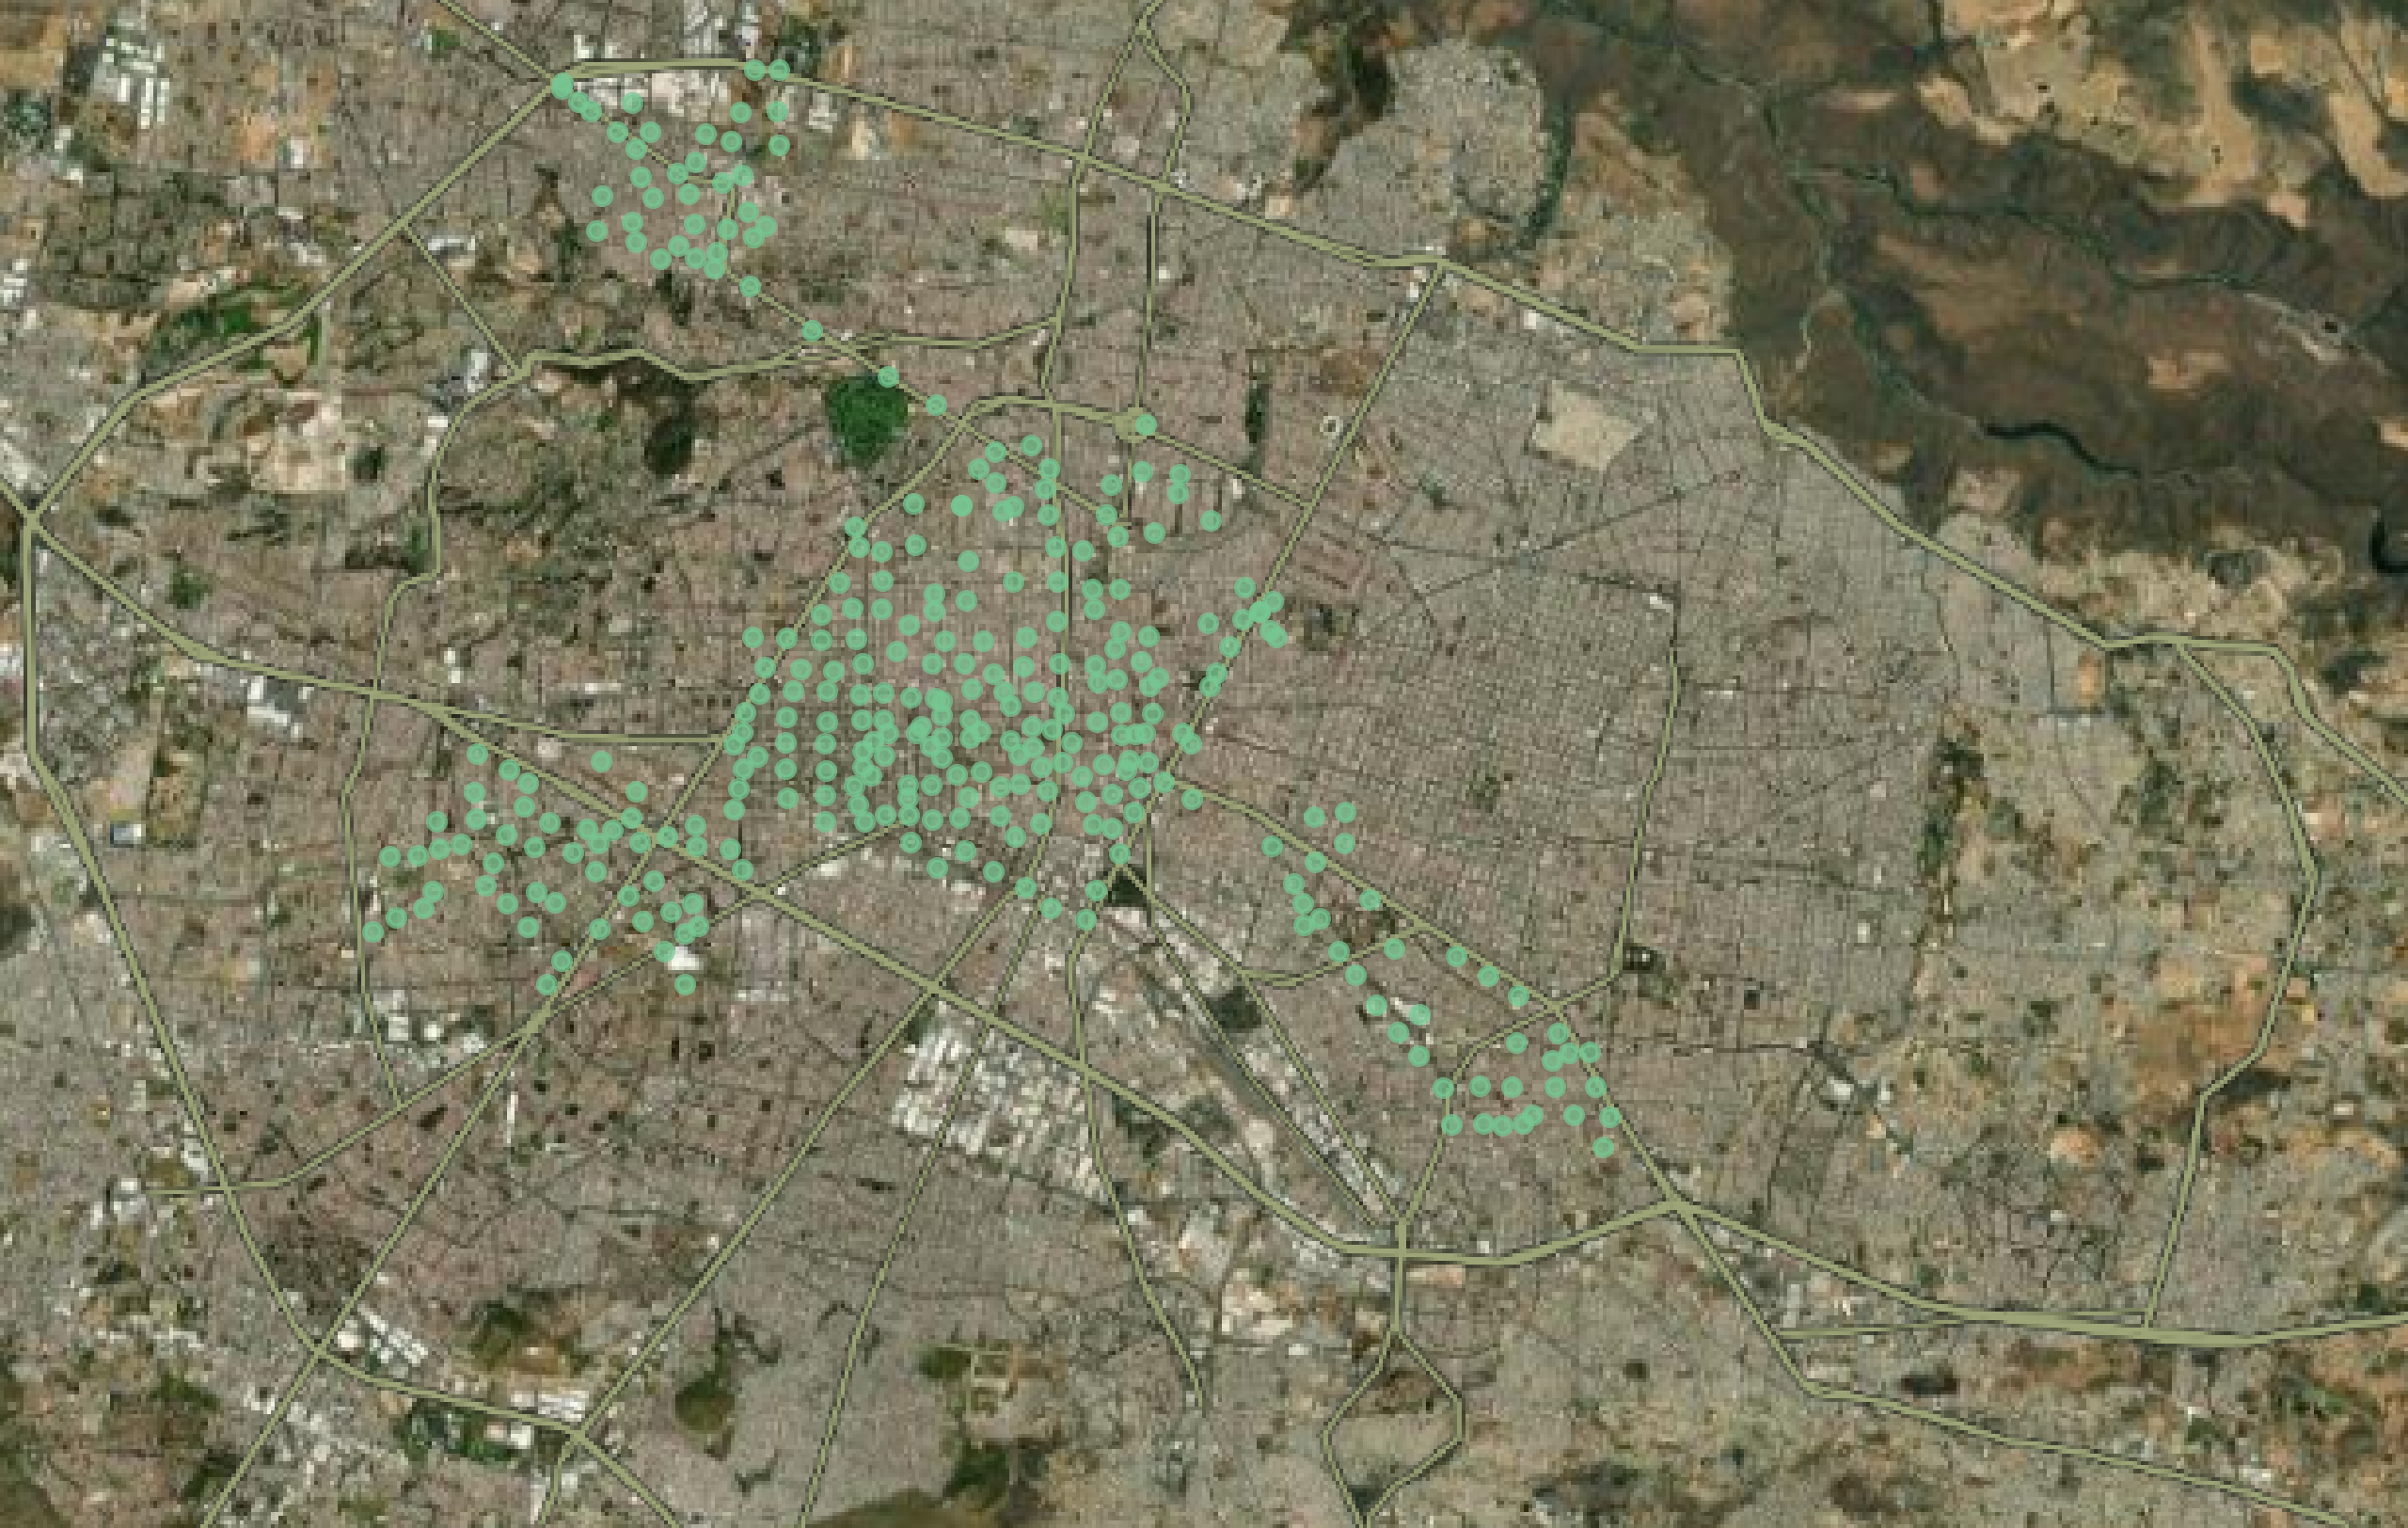
\includegraphics[width=12cm,height=5cm]{Graphics/stations.png}
    \caption{Localización de las estaciones de MIBICI en la ciudad de Guadalajara.}
    \label{fig:MIBICI_stations}
\end{figure}
% \begin{table}[H]
%     \centering
%     \begin{tabular}{lccccc} \hline
%                                          & \textbf{Automovil} & \textbf{Autobús} & \textbf{Bicicleta} & \textbf{Avión} & \textbf{Tren} \\ \hline
%         Consumo de espacio               & 100\%              & 10\%             & 8\%                & 1\%            & 6\%           \\
%         Consumo de energía primaria      & 100\%              & 30\%             & 0\%                & 405\%          & 34\%          \\
%         Emisiones CO\textsubscript{2}    & 100\%              & 29\%             & 0\%                & 420\%          & 4\%           \\
%         Emisiones NO\textsubscript{x}    & 100\%              & 9\%              & 0\%                & 290\%          & 4\%           \\
%         Emisiones CO                     & 100\%              & 2\%              & 0\%                & 93\%           & 1\%           \\
%         Contaminacipin atmosférica total & 100\%              & 9\%              & 0\%                & 250\%          & 3\%           \\
%         Riesgo inducido de accidente     & 100\%              & 9\%              & 2\%                & 12\%           & 3\%           \\ \hline
%     \end{tabular}
%     \caption{Comparación entre el vehículo privado y distintos medios de transporte para diversos indicadores medioambientales\cite{dekoster_2000}.}
% \end{table}